\documentclass[11pt]{article}
\usepackage[a4paper,margin=1in]{geometry}
\usepackage{fontspec}
\newfontfamily\cjkfont{Noto Serif CJK SC}
\newcommand{\cn}[1]{{\cjkfont #1}}
\usepackage{graphicx}
\usepackage{amsmath}
\usepackage{microtype}
\usepackage{caption}
\captionsetup{font=small,labelfont=bf}
\usepackage[super,comma,sort&compress]{natbib}
\usepackage{xcolor}
\definecolor{linkblue}{RGB}{0,84,166}
\definecolor{thupurple}{RGB}{102,8,116}
\usepackage{hyperref}
\hypersetup{colorlinks=true, urlcolor=linkblue, linkcolor=linkblue, citecolor=black,
  pdftitle={Designing, Commercializing and Internationalizing Chinese Spherical Tokamaks}, pdfauthor={Jony}}
\newcommand{\jl}[2]{\href{#2}{#1}}
\setlength{\parindent}{1.4em}
\setlength{\parskip}{0.15em}
\begin{document}

\begin{titlepage}
\centering
\vspace*{0.7cm}

\includegraphics[width=0.46\textwidth]{assets/tsinghua_logo.png}\\[1.0cm]
{\large\color{thupurple}\scshape Tsinghua University}\\[0.20cm]
{\normalsize Department of Engineering Physics\\[2pt]
Nuclear Engineering and Management (TUNEM)}\\[1.5cm]
{\color{thupurple}\rule{0.82\textwidth}{1.1pt}}\\[0.35cm]
{\large THESIS PROPOSAL}\\[0.5cm]
{\LARGE\bfseries Designing, Commercializing and\\[0.25cm]
Internationalizing Chinese Spherical Tokamaks}\\[0.45cm]
{\large\itshape A Unified Three-Case Study of Spherical-Tokamak Fusion in China}\\[0.32cm]
{\color{thupurple}\rule{0.82\textwidth}{1.1pt}}\\[1.6cm]
{\large
\begin{tabular}{rl}
Name: & \cn{乔纳森}~(Jony), TUNEM Student\\[0.32cm]
Academic Advisor: & \cn{谭熠}~(Tan Yi), Tsinghua University\\[0.32cm]
Industry Advisor: & \cn{叶成}~(Ye Cheng), SNERDI\\
\end{tabular}}\\[1.6cm]
{\large June 26, 2026}
\vfill
\end{titlepage}

\clearpage

\thispagestyle{plain}
\phantomsection\addcontentsline{toc}{section}{\texorpdfstring{\cn{摘要}}{Zhaiyao} (Chinese Abstract)}
{\cjkfont
\XeTeXlinebreaklocale "zh"
\XeTeXlinebreakskip=0pt plus 1pt
\begin{center}{\Large\bfseries 摘\quad 要}\end{center}
\vspace{0.3em}

\setlength{\parindent}{2em}
本研究以清华大学核能与管理项目（TUNEM）的使命——培养能够连接中国核能事业与各国发展需求的国际化核能管理人才——为出发点，旨在为有志于推动中国聚变能“走出去”的工程师型创业者撰写一份可操作的“实践蓝图”。论文以球形托卡马克聚变为研究对象，通过三个案例并在“能力 $\rightarrow$ 商业化 $\rightarrow$ 国际市场”的统一框架下展开：（一）以 SUNIST-2 为例，梳理紧凑型球形托卡马克反应堆的物理与工程要点；（二）以 Startorus（星环聚能）为例，分析这一技术能力如何转化为可融资、可监管的企业；（三）以上海核工程研究设计院（SNERDI）的国际经验为参照，探讨何种国际化路径能够把这类中国清洁能源技术带向巴西、南非、土耳其等伙伴国家。本文的意义不在于技术创新，而在于\textbf{社会效益与全球能源合作}：清洁、充裕的基荷电力是发展中国家发展的关键支点；以合作而非攫取的方式将其落地，既服务于中国的能源外交，也促进伙伴国家的共同发展。

\vspace{0.7em}
\noindent\textbf{关键词：}\ 球形托卡马克；聚变能；商业化；国际化；能源合作；共同发展
\par}
\setlength{\parindent}{1.4em}

\clearpage

\phantomsection\addcontentsline{toc}{section}{Table of Contents}
\renewcommand{\contentsname}{Table of Contents}
\tableofcontents
\clearpage

\phantomsection\addcontentsline{toc}{section}{Executive Summary}
\begin{center}
{\large\textbf{Executive Summary}}\\[2pt]
{\small Designing, Commercializing and Internationalizing Chinese Spherical Tokamaks --- TUNEM Master's Research Proposal}
\end{center}
\vspace{2pt}

This proposal advances four core claims along one spine --- Capabilities $\rightarrow$ Commercialization $\rightarrow$ International Markets; the first two are technical and form the analytical heart of the thesis.

\textbf{1.~Reconstructing the design interface.} Freidberg, Mangiarotti and Minervini's \emph{Designing a Tokamak Fusion Reactor---How Does Plasma Physics Fit In?} (Phys.\ Plasmas, 2015) shows that a reactor's main parameters are fixed almost entirely by nuclear and engineering constraints, leaving the plasma to satisfy a small set of coupled limits. The thesis derives that ``design interface'' from first principles --- the knobs (field $B$, shape and $\beta$, heating, pulse) and the operational limits (Troyon, Greenwald, kink, bootstrap) that bind them --- rebuilding transparently what the specialist sources compress or assume.

\textbf{2.~Deriving the spherical tokamak as the route that closes Freidberg's constraints.} Freidberg derives that a conventional tokamak does not close: the required plasma current exceeds the kink limit, and the achievable bootstrap fraction ($\approx 0.44$) falls short of the value steady state requires ($\approx 0.84$). One of his own remedies is to raise the magnetic field --- which lowers the required current and eases the kink limit --- and the spherical tokamak reaches that same high-field-favourable regime through \emph{geometry}. Two distinct mechanisms do the work, kept separate: the ST's strong $\tau_E\propto B^{1.0}$ scaling lets confinement come from field rather than current, relieving the kink/current trap, while its low aspect ratio raises the trapped-particle (bootstrap) fraction, relieving the bootstrap shortfall directly; high $\beta$ is then an economic and stability margin, not the cure. The spherical-tokamak reactor literature (Peng; Sykes; Menard) develops low-aspect-ratio designs in the high-bootstrap, high-field regime, but does not engage Freidberg's closure argument; connecting that regime to his specific over-constraint --- showing transparently that the ST relieves the two failure modes he identifies --- is this thesis's own \emph{synthesis}, accessible exposition rather than new physics.

\textbf{3.~Commercialization --- the core product problem.} The heart of commercializing a reactor is making a useful product people will pay for, and \emph{scientific} breakeven is not economic viability. The thesis derives that gap --- separating what the spherical tokamak has \emph{demonstrated} (high $\beta$, bootstrap fraction, compactness) from the hard walls that \emph{remain} (sustained high-field confinement, tritium breeding in cramped geometry, neutron-tolerant materials, continuous operation) --- and frames it as the directed engineering agenda the entrepreneur must close before a commercial product exists. Capital, regulation, supply chain and the other hurdles of building a fusion company are taken up only \emph{after} that core product problem, at literature-review depth on public sources.

\textbf{4.~Internationalization --- taking the technology abroad.} The thesis closes by asking what deal structures could carry a Chinese energy technology to partner countries. Five engagements --- Pakistan, Argentina, Turkey, South Africa and Brazil --- yield a diagnostic of buyer-side conditions: energy demand, political continuity, financing capacity, and local diversification. SNERDI's design and licensing work on CAP1400 and CNP-300 offers the institutional template; CNNC's Hualong One in Pakistan offers the success model. This integrated synthesis --- absent from a literature that is either specialist or business-only --- is what makes TUNEM's engineering-and-management mission concrete as an actionable blueprint for the engineer-entrepreneur, and it is the foundation of the author's intended post-doctoral ventures.

\textbf{Primary sources.} The analytical core rests on Freidberg, Mangiarotti \& Minervini (2015); Freidberg, \emph{Plasma Physics and Fusion Energy}; Wesson, \emph{Tokamaks}; the spherical-tokamak reactor literature (Peng; Sykes; Menard); and Prof.\ Tan Yi's SUNIST-2 programme, whose stated aims --- confinement at higher \emph{magnetic field}, magnetic-reconnection heating, plasma-shaping and control, and repetitive pulsed operation --- map directly onto the design knobs, the field knob above all.
\clearpage

\bigskip

% =====================================================================
\phantomsection\addcontentsline{toc}{section}{a.~~Significance of the Topic}\section*{a.~~Significance of the Topic}
% =====================================================================
Controlled \jl{nuclear fusion}{https://en.wikipedia.org/wiki/Nuclear_fusion} --- the reaction that powers the Sun --- has promised abundant, clean and inherently safe energy for seventy years, yet has always seemed ``thirty years away.'' Two developments have moved it from a purely scientific quest to an engineering-and-business race. The first is the maturing of \jl{high-temperature superconducting}{https://en.wikipedia.org/wiki/High-temperature_superconductivity} (HTS) magnets, which allow a strong magnetic field --- and therefore a fusion-relevant plasma --- in a much smaller machine.\cite{costley2019,sykes2018} The second is a surge of private capital, in which China has become a central arena. The question is no longer only \emph{whether} fusion works, but \emph{how} a device is built, commercialized, and ultimately sold.

Most accounts answer only one part of that question. Physicists describe the reactor; investors describe the deal; policy analysts describe the strategy. Very few connect, end to end, how a specific reactor is actually built, how that engineering capability becomes a fundable company, and how such a company might go global. This thesis proposes exactly that integrated account, following one real lineage: the \jl{SUNIST-2 spherical tokamak}{https://en.wikipedia.org/wiki/Spherical_tokamak} built at Tsinghua University, the start-up \jl{Startorus Fusion}{https://startorus.com/process/} it seeded, and the international-energy experience of \jl{SNERDI}{https://www.snerdi.com.cn/}. The unifying lens is a three-layer pathway --- \textbf{Capabilities $\rightarrow$ Commercialization $\rightarrow$ International Markets} --- through which the three cases are read as one story.

This is the kind of boundary-spanning work the TUNEM programme exists to produce. A study that follows a device from the laboratory bench (engineering) to the enterprise (management) to foreign markets (international business) sits precisely at the nuclear-engineering--and--management intersection. It is also honest about its author's vantage: my training is in mathematics and entrepreneurship, not yet engineering, so the intended contribution is not novel engineering constructs but a structured, candid synthesis --- a \emph{blueprint} a future engineer-entrepreneur could actually use to materialize TUNEM's stated mission. What physical and engineering choices define a compact spherical-tokamak reactor? What do those choices cost and what do they de-risk? How is a Chinese deep-tech fusion venture regulated, organized and realized? And what does the internationalization of Chinese energy firms teach about taking nuclear energy abroad? Direct access to the two principals --- Prof.\ Tan Yi, who built SUNIST-2 and founded Startorus, and Ye Cheng of SNERDI --- makes primary-source grounding feasible.

This proposal does not attempt to master every engineering detail; that is the work of the thesis itself. Section~b.1 establishes the core principles that motivate the spherical tokamak and the SUNIST-2 design at a level a non-specialist can follow, and marks where the thesis will go deeper: a \emph{physics-guided design philosophy} relating the knobs one can turn --- field, shape, heating, pulse scheme --- to the engineering and material constraints that bound them.

% =====================================================================
\phantomsection\addcontentsline{toc}{section}{b.~~Literature Review}\section*{b.~~Literature Review}
% =====================================================================
The review proceeds in three strands: (b.1)~the physics and engineering of spherical tokamaks and SUNIST-2; (b.2)~the commercialization of fusion, from the engineering-breakeven problem of a profitable reactor to the demands beyond it; and (b.3)~the internationalization of Chinese energy firms. This draft develops the first and most technical strand, the foundation on which Cases~2 and~3 build.

\phantomsection\addcontentsline{toc}{subsection}{b.1~~Spherical-Tokamak and SUNIST-2 Physics and Engineering}\subsection*{b.1~~Spherical-Tokamak and SUNIST-2 Physics and Engineering}

This strand follows the account given by the SUNIST-2 team's own publications --- in particular Tan and Gao's recent device overview\cite{tan_iaea} and the equilibrium-design study of Cheng, Gao and Tan\cite{cheng2022}, together with the team's earlier Chinese-language work on the SUNIST lineage\cite{sunist_cn2004,tan_gao2010_cn,tan_phd2009} --- and uses the wider spherical-tokamak literature to corroborate, claim by claim, the statements those sources (and Tsinghua's and Startorus's public materials) make without going into the underlying technical reality. The path is set by Prof.\ Tan Yi and SUNIST-2; the outside references supply the independent backing.

\paragraph{(i)~What fusion demands.}
Fusion releases energy when two light nuclei --- in the easiest case the hydrogen isotopes \jl{deuterium}{https://en.wikipedia.org/wiki/Deuterium} and \jl{tritium}{https://en.wikipedia.org/wiki/Tritium} --- merge into a heavier one. The difficulty is that nuclei are positively charged and repel each other through the \jl{Coulomb barrier}{https://en.wikipedia.org/wiki/Coulomb_barrier}; only at enormous speeds do they collide closely enough to fuse. In practice this means heating the fuel above $100$~million~$^\circ$C, hotter than the Sun's core, at which point matter becomes a \jl{plasma}{https://en.wikipedia.org/wiki/Plasma_(physics)} --- a gas of free electrons and ions.\cite{freidberg,wesson} No material wall can hold such a plasma, so it must be suspended away from every surface. The condition for net energy, the \jl{Lawson criterion}{https://en.wikipedia.org/wiki/Lawson_criterion} (often stated as a ``triple product'' of density, temperature and energy-confinement time), says the plasma must be simultaneously hot enough, dense enough, and held together long enough.\cite{lawson1957} Meeting that triple target is the central engineering problem of magnetic fusion.

\paragraph{(ii)~Why magnetic confinement, and why a torus.}
Because a plasma is electrically charged, its particles spiral along magnetic-field lines: a magnetic field is therefore an invisible bottle that can keep the hot plasma off the walls.\cite{freidberg} A straight bottle leaks at its ends, so the field is bent into a closed ring --- a \jl{torus}{https://en.wikipedia.org/wiki/Torus} --- with no ends to leak from. A purely \jl{toroidal field}{https://www.energyencyclopedia.com/en/nuclear-fusion/tokamaks/toroidal-field} (the long way around the ring) is stronger on the inside than the outside, which makes particles drift outward; the cure is to add a \jl{poloidal field}{https://www.energyencyclopedia.com/en/nuclear-fusion/tokamaks/poloidal-field} (the short way around) so the field lines become helical and the drifts average out. The \jl{tokamak}{https://www.energyencyclopedia.com/en/nuclear-fusion/tokamaks} produces that poloidal field by driving a large electric current through the plasma itself, induced like the secondary of a transformer by a \jl{central solenoid}{https://www.energyencyclopedia.com/en/nuclear-fusion/tokamaks/central-solenoid}. A tokamak is thus described by a few numbers used throughout this thesis: the major radius $R$ (the size of the ring), the minor radius $a$ (the thickness of the tube), their ratio the \emph{aspect ratio} $A=R/a$, the magnetic field $B$ (measured in \jl{tesla}{https://en.wikipedia.org/wiki/Tesla_(unit)}), and the plasma current. Figure~\ref{fig:iter} labels these on a conventional machine.

\begin{figure}[t]
\centering
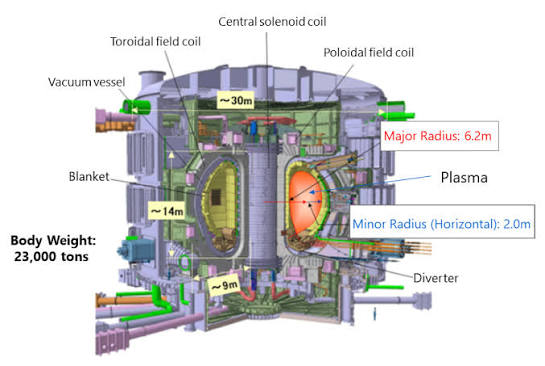
\includegraphics[width=0.66\linewidth]{assets/img_toshiba.jpeg}
\caption{Anatomy of a conventional (large-aspect-ratio) tokamak, ITER, labelling the toroidal-field coils, central solenoid, poloidal-field coils, vacuum vessel, blanket and divertor, with major radius $6.2$~m and minor radius $2.0$~m. SUNIST-2 uses the same components at about one-twelfth of ITER's major radius ($0.53$~m versus $6.2$~m). Figure source: \jl{Toshiba}{https://www.toshiba-clip.com/en/detail/p=482} (ITER cut-away and dimensions); reproduced for educational use.}
\label{fig:iter}
\end{figure}

\paragraph{(iii)~Why ``spherical''---the shape choice and its physics payoff.}
A conventional tokamak is a fat doughnut with $A\approx 3$. If one pushes the central hole nearly shut, the doughnut becomes a cored apple: a \emph{spherical tokamak} (ST) with $A<2$, a configuration first analysed by Peng and Strickler.\cite{peng1986} The shape pays off physically in several ways. The most important is high \jl{beta}{https://en.wikipedia.org/wiki/Beta_(plasma_physics)} ($\beta$), the ratio of plasma pressure to magnetic pressure --- a measure of how efficiently the field is used. Since fusion power scales with \emph{absolute} pressure ($P_{\mathrm{fus}}\propto\beta^{2}B^{4}$), a high $\beta$ raises power for a given field but does not replace it; the spherical-tokamak bet is to reach high absolute pressure in a small machine once the field is raised. STs reach $\beta$ far above conventional tokamaks: record toroidal $\beta>30\%$ on START --- more than twice the $12.6\%$ DIII-D record --- and a transient $\approx 60\%$ in plasma-merging (TS-3/4) experiments, versus around $12\%$ in conventional devices.\cite{sykes1997,tan_iaea} Because fusion power scales steeply as $P_{\mathrm{fus}}\propto R^{3}B^{4}\beta^{2}$, a high-$\beta$ machine can reach reactor conditions at smaller size and lower field --- the central argument for cheaper, faster-to-build reactors.\cite{sykes2018,tan_iaea} STs also show energy confinement improving strongly with field, a large self-generated \jl{bootstrap current}{https://en.wikipedia.org/wiki/Bootstrap_current} that reduces the external current that must be driven, and a favourable \jl{divertor}{https://en.wikipedia.org/wiki/Divertor} heat-load geometry.\cite{tan_iaea,costley2019}

Honesty requires the catch. Squeezing the hole shut leaves the central column cramped, with little room for the solenoid that normally starts and sustains the current, for neutron shielding, or --- in a power plant --- for a durable magnet. And the favourable confinement scalings are measured almost entirely below $1$~T; only ST40 has operated above it, at $2.2$~T.\cite{tan_iaea,mcnamara2024} These constraints are not footnotes: they \emph{are} the engineering agenda of the spherical tokamak, and they define what SUNIST-2 was built to study.

\paragraph{(iv)~The distinguishing engineering choices, embodied in SUNIST-2.}
SUNIST-2 is a compact ST with major radius $R_0=0.53$~m, minor radius $a=0.33$~m, on-axis field $B=1.0$~T and a design plasma current of $0.5$~MA; it achieved first plasma in 2023 and has since reached $480$~kA.\cite{tan_iaea,sunist2design2025,cheng2022} Figure~\ref{fig:sunist} shows the machine. Each of its signature choices answers one of the ST challenges above.

\begin{figure}[t]
\centering
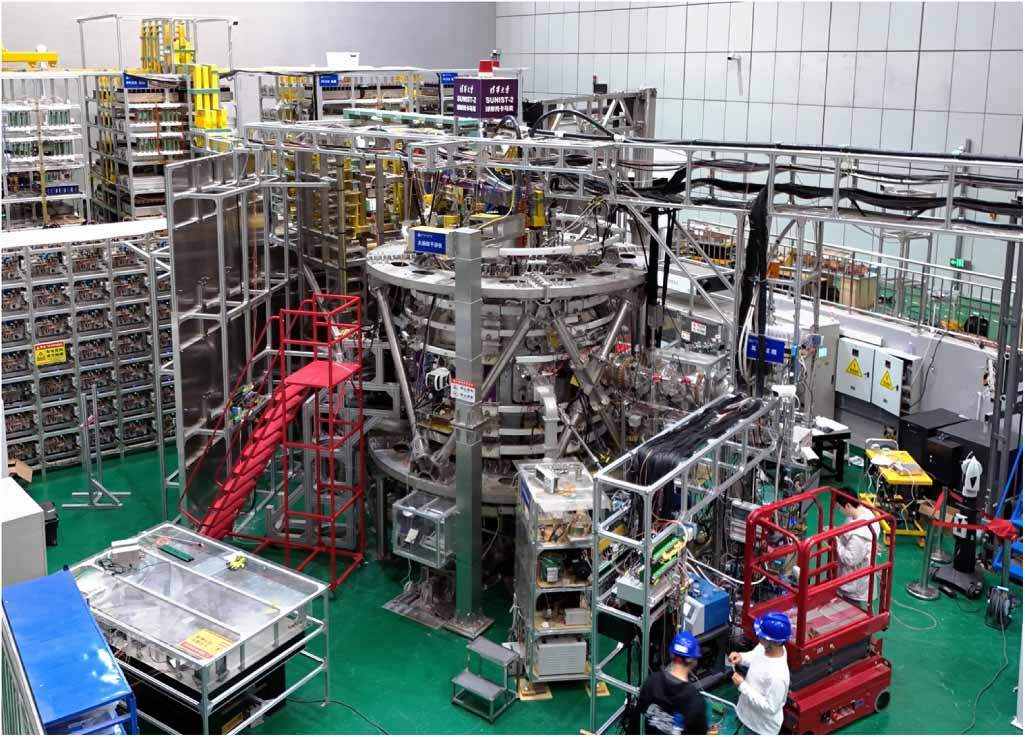
\includegraphics[width=0.62\linewidth]{assets/img_sunist2_ae1533.jpg}
\caption{The SUNIST-2 spherical tokamak at Tsinghua University: the central column and vacuum vessel (centre) surrounded by the support structure, with the modular capacitor-based magnet power supplies at left. Source: SUNIST-2 magnetic-plasma-control study, \emph{Plasma Phys.\ Control.\ Fusion} (2024),\cite{sunist2control2024} via \jl{iopscience.iop.org/.../ae1533}{https://iopscience.iop.org/article/10.1088/1361-6587/ae1533}.}
\label{fig:sunist}
\end{figure}

\emph{Solenoid-light startup.} Because the central column cannot host a large solenoid, SUNIST-2 explores starting the plasma without leaning on one --- forming two plasma rings and letting them merge (``merging-compression''), assisted by a plasma gun, to economise the limited magnetic flux.\cite{tan_iaea} \emph{Magnetic-reconnection heating.} When the two rings merge, their fields undergo \jl{magnetic reconnection}{https://en.wikipedia.org/wiki/Magnetic_reconnection}, converting stored magnetic energy directly into ion heat, with heating that grows as the square of the plasma current. This heating-by-startup, studied earlier on the TS-3/4 and MAST devices, is SUNIST-2's signature physics.\cite{ono2015,tanabe2015,tan_iaea} \emph{Plasma shaping and negative triangularity.} An active control system shapes the plasma to a ``triangularity'' as large as $\pm0.6$. Negative triangularity is of special interest because it can deliver high-confinement performance while remaining free of the damaging edge bursts called \jl{edge-localized modes}{https://en.wikipedia.org/wiki/Edge-localized_mode} (ELMs), easing the load on a reactor wall.\cite{nelson2024,camenen2007,sunist2control2024} SUNIST-2's own equilibrium-design work, using a free-boundary code adapted from EFIT, maps which plasma shapes --- limiter, double-null and negative-triangularity configurations --- are reachable and sizes the poloidal-field power supply needed to produce them.\cite{cheng2022} \emph{Repetitive pulsed operation.} Rather than one long pulse, SUNIST-2 has demonstrated dual-pulse operation --- the seed of an ``engine-like'' repetitive scheme the company intends to scale.\cite{tan_iaea} \emph{Magnets and materials.} SUNIST-2 uses copper coils today; the commercial concept migrates to HTS magnets for high field in a compact volume.\cite{costley2019,sykes2018} \emph{Wall conditioning.} Coating the vessel wall with lithium sharply reduced carbon and oxygen impurities, a simple but consequential operational technique.\cite{tan_iaea} Finally, the engineering is increasingly \emph{predicted before it is built}: a plasma burn-through code reproduced SUNIST-2 (and EAST) start-up to within about $15\%$, illustrating the model-then-build discipline the thesis will examine.\cite{li2025}

\paragraph{(v)~Safety and protection.}
Fusion is inherently safe in a way fission is not: there is no chain reaction, only seconds of fuel sit in the vessel at any moment, and almost any disturbance cools the plasma and stops the reaction --- it fails safe, with no possibility of meltdown.\cite{freidberg} But a real machine still has hazards that must be engineered for, and they belong in any honest ``how to build it'' account. The foremost is the \emph{disruption}: a sudden, uncontrolled collapse of confinement that dumps the plasma's energy and current into the vessel, exerting large electromagnetic forces and, in large machines, generating high-energy ``runaway'' electrons that can pierce the wall; predicting, avoiding and mitigating disruptions (for example by massive gas or pellet injection) is a central safety task.\cite{hender2007,boozer2012} Tritium fuel is radioactive and must be handled and accounted for under regulation; the energetic \jl{neutrons}{https://en.wikipedia.org/wiki/Neutron} from D--T fusion activate structural materials, demanding shielding and low-activation steels; and the large stored magnetic and electrical energy (coil currents, capacitor banks, and \jl{magnet quench}{https://en.wikipedia.org/wiki/Superconducting_magnet} in HTS systems) must be safely dissipated. For a compact ST the safety arithmetic partly eases --- smaller stored energy and lower absolute currents than ITER --- and partly sharpens, because the same power flows through a tighter space. The thesis will treat the ST safety case as part of the design philosophy, not an afterthought.\cite{tan_iaea,hender2007}

\paragraph{(vi)~Synthesis and what the thesis will deepen.}
The literature reviewed here tells a coherent story. Foundational ST physics\cite{peng1986,sykes1997} explains \emph{why} the spherical shape is attractive; modern high-field and shaping results\cite{mcnamara2024,nelson2024} show how far the concept has come and where it is still unproven; reconnection-heating studies\cite{ono2015,tanabe2015} ground SUNIST-2's distinctive heating route; and the SUNIST-2 papers themselves\cite{tan_iaea,cheng2022,li2025,sunist2design2025,sunist2control2024} document a deliberately compact, low-cost, fast-iterating machine built to probe exactly the open questions --- high-field confinement, solenoid-free start-up, reconnection heating, repetitive operation --- that a commercial ST reactor must answer. It is, in short, the technical seed of Startorus's reactor concept and the natural anchor of Case~1. The thesis will turn this review into a physics-guided design philosophy: for each performance knob --- field $B$, shape and $\beta$, heating method, pulse scheme --- what it buys, which engineering or material constraint bounds it, and how SUNIST-2's particular choices trade among them. Paywalled SUNIST-2 engineering detail, notably the full preliminary-design paper,\cite{sunist2design2025} will be incorporated as it is obtained.

% =====================================================================

\bigskip

\phantomsection\addcontentsline{toc}{subsection}{b.2~~Closing the Reactor: From the Design Interface to a Profitable Spherical Tokamak}\subsection*{b.2~~Closing the Reactor: From the Design Interface to a Profitable Spherical Tokamak}

The error this section sets out to correct is the quiet assumption that commercializing fusion is, at heart, a financing story. It is not. The crux of commercialization is a reactor that yields abundant clean energy from a little fuel --- the product fusion has failed to deliver for seventy years --- and capital, regulation, talent and supply chains are downstream of that. Section~b.1 built a physics-based design interface: the knobs (magnetic field $B$, plasma shape and beta $\beta$, heating method, pulse scheme) and the limits that couple them. Here that interface does real work, in three movements. First (b.2.1a) it is applied to derive, accessibly, why the conventional tokamak does not close as a reactor. Then (b.2.1b) the spherical tokamak appears as the escape that attacks exactly that closure problem --- followed by the ST's own hard walls and the engineering-breakeven barrier every approach shares. Finally (b.2.2) the downstream commercialization demands are reviewed briefly and in a Chinese frame. The depth throughout is that of a literature review; the thesis itself goes operational through the Startorus case.

\paragraph{b.2.1a~~Applying the interface: why the conventional tokamak does not close.}
Freidberg, Mangiarotti and Minervini show that a tokamak reactor's main parameters are fixed almost entirely by nuclear physics and engineering, with plasma physics entering decisively in only one place.\cite{freidberg2015} Read through b.1's knobs, the logic is intuitive. The deuterium--tritium reaction rate peaks near $15$~keV, which fixes the temperature; the fusion power density and the neutron load the first wall can survive fix the pressure, field and size; the breeding blanket's roughly one-metre thickness fixes the major radius. With these alone, the minor radius $a$, major radius $R_0$, field $B_0$, temperature, pressure, density and the required energy-confinement time $\tau_E$ follow with almost no plasma physics. The exception is the plasma \emph{current}. The confinement the design demands requires a large current, but the plasma's own ceilings --- the \jl{Troyon}{https://en.wikipedia.org/wiki/Beta_(plasma_physics)} $\beta$ limit,\cite{troyon1984} the Greenwald density limit,\cite{greenwald1988} the kink-stability (safety-factor) limit, and the \jl{bootstrap-current}{https://en.wikipedia.org/wiki/Bootstrap_current} fraction limit\cite{kikuchi1990} --- cannot supply it. Freidberg's reference reactor fails in two ways at once: the required current exceeds the kink disruption limit, and the achievable bootstrap fraction (about $0.44$) falls well short of the value the steady-state design requires (about $0.84$), so even bootstrap current plus external current drive cannot sustain it.\cite{freidberg2015} The reactor is therefore over-constrained: it does not close. The honest statement is ``severely over-constrained under standard assumptions,'' not ``impossible'' --- and Freidberg's own resolution points two ways, to advances in plasma physics that raise $\beta$ and confinement, or to engineering that raises the magnetic field.\cite{freidberg2015} This is the payoff of the b.1 interface: the same knobs, pushed through four inequalities, yield a real reactor's feasibility verdict, made legible without the specialist apparatus the original assumes.

\paragraph{b.2.1b~~The spherical-tokamak escape, and its own walls.}
Freidberg's own remedies are to raise the field with high-temperature superconductors, or to retreat to the stellarator or the fusion--fission hybrid; he treats raising $\beta$ through advanced plasma-physics profile control as risky, and does not consider the \jl{spherical tokamak}{https://en.wikipedia.org/wiki/Spherical_tokamak} (ST) at all.\cite{freidberg2015} Yet the ST reaches his preferred high-field-favourable regime through \emph{geometry}, and the physics by which a low-aspect-ratio device can operate as a reactor is itself a substantial literature.\cite{peng1986,sykes2018,menard2016} It attacks his two failure modes directly --- and does more. Squeezing the aspect ratio below two raises $\beta$ sharply: START reached toroidal $\beta>30\%$, more than twice the previous tokamak record of $12.6\%$ on DIII-D, and later STs such as NSTX and MAST routinely exceed $30\%$; since fusion power scales as $P_{\mathrm{fus}}\propto R^{3}B^{4}\beta^{2}$, that buys reactor conditions at smaller size and lower field.\cite{sykes1997,tan_iaea} More pointedly, the ST attacks the exact failure that broke the reference design: its pronounced toroidicity traps a large fraction of particles, producing a high bootstrap-current fraction that supplies much of the plasma current internally and slashes the external current-drive demand.\cite{tan_iaea} And ST confinement scales as $\tau_E\propto B^{1.0}$, against $B^{0.15}$ for a conventional tokamak, so an ST reactor is pushed to raise the \emph{field} rather than the \emph{current} --- avoiding precisely the high-current, disruption-prone regime that over-constrained the conventional machine.\cite{tan_iaea,mcnamara2024} The ST thus relaxes both of Freidberg's failure modes at once --- the kink/current trap (via the $\tau_E\propto B$ scaling, confinement from field rather than current) and the bootstrap shortfall (via low aspect ratio) --- with high $\beta$ a further bonus rather than the cure. Deriving that closure transparently, on the foundation of the ST-reactor literature, is the move this thesis makes for Case~1.\cite{menard2016,sykes2018,costley2019} But geometry does not make the field free: the structural-stress penalty Freidberg attaches to raising the field --- in his words ``substantially more structural'' material at the inboard side --- reappears in the spherical tokamak concentrated onto its cramped, poorly shielded \emph{centre stack}, so the configuration \emph{relocates} that cost rather than escaping it. Whether the geometric gains in $\beta$ and bootstrap outweigh the centre-stack penalty at reactor scale is the open question Case~1 frames --- and it is precisely what SUNIST-2's signature choices (a segmented central solenoid, merging-compression startup, reconnection heating) are built to probe.\cite{tan_iaea}

Reality pushes back again, now in ST-specific ways the SUNIST-2 team states plainly.\cite{tan_iaea} First, the favourable confinement scalings are measured almost entirely below $1$~T; only ST40 has run higher, at $2.2$~T, so whether the strong $\tau_E$--$B$ scaling survives to reactor fields is unverified.\cite{mcnamara2024} Second, the compact central column severely limits the available magnetic flux, making plasma initiation and long-pulse operation hard, while the ST's high plasma dielectric constant impedes the lower-hybrid current drive used in conventional tokamaks --- forcing ST-specific operating scenarios. Third, neutral-beam injection is the only well-demonstrated ST heating, leaving efficient ion heating suited to ST geometry an open problem. These three challenges map one-to-one onto SUNIST-2's three stated aims --- confinement at higher field, ion heating by magnetic reconnection, and repetitive pulsed operation --- so the device is purpose-built to attack exactly the ST's open questions; its merging-compression startup, segmented central solenoid and reconnection heating are research moves at these very walls.\cite{tan_iaea,cheng2022,li2025}

Beneath the ST's own problems lies the wall every approach shares, and the one that actually decides profitability: \jl{engineering breakeven}{https://en.wikipedia.org/wiki/Fusion_energy_gain_factor}. Producing more fusion energy than is delivered to the fuel --- scientific breakeven, $Q\ge1$ --- has been demonstrated in inertial confinement (the National Ignition Facility reached target gain in 2022) but not yet in magnetic confinement: JET's deuterium--tritium record reached only $Q\approx0.67$, no spherical tokamak has approached $Q\approx1$, and ITER is designed for $Q=10$.\cite{abushawareb2024,keilhacker1999,wurzel_hsu2022} What no device has reached is engineering breakeven --- net electricity exceeding the \emph{total} electricity to run the plant, including cryogenics, magnets, heating and balance-of-plant --- which is why a commercial reactor must reach $Q$ of order $10$--$30$, not $1$.\cite{wurzel_hsu2022,costley2019} Beyond that lies economic viability at a competitive cost of electricity, further still. The remaining barriers are engineering and materials, not whether fusion can occur: \jl{tritium}{https://en.wikipedia.org/wiki/Tritium} self-sufficiency (a D--T plant must breed its own tritium from lithium with a breeding ratio above one, unproven at scale and especially hard in the cramped ST column),\cite{abdou2006} first-wall survival under $14$~MeV neutron damage (no material yet endures power-plant fluence economically),\cite{zinkle_snead2014} and continuous, disruption-free operation.\cite{hender2007} An honest ledger for the ST: high $\beta$, compactness and a high bootstrap fraction are demonstrated; sustained high-field confinement, breeding and shielding in cramped geometry, and net electricity are not. That gap is the frontier SUNIST-2 and Startorus occupy.

\paragraph{b.2.2~~Downstream: what commercialization additionally requires.}
Only once a profitable reactor is in sight do the remaining demands bind, and they are downstream of --- not equivalent to --- the product problem. At review depth: deep-technology ventures like fusion must cross a long, capital-hungry ``valley of death'' that ordinary venture funding handles poorly, so patient and public capital matter.\cite{fia2025} But in China this is shaped less by the venture-and-IPO arc of Western accounts than by state-backed capital and national strategy; the domestic regulatory framework for fusion is still being built; and the supply chain for fusion-grade hardware --- high-field magnets, pulsed-power systems, diagnostics --- is itself a venture-defining problem of where such components are obtained and by whom they are qualified.\cite{xinhua2025,tan_interview_cn,chenrui_interview_cn} These are real and necessary, but subordinate to the net-energy problem above; the thesis treats them operationally through the Startorus case, whereas here they are reviewed and bounded rather than narrated. Two scoping points follow. First, the treatment is deliberately \emph{general and structural} --- the commercialization \emph{patterns} (capital, regulation, supply chain), not any single firm's confidential financials or internal strategy --- and it draws only on the public record. Second, that the scholarly literature on commercializing a Chinese fusion venture is still thin is not a reason to avoid the question but a reason to pursue it: an under-served area is precisely where a careful, public-source synthesis contributes most.

\paragraph{Synthesis and the gap.}
The literature closes pieces of this chain but not the chain itself. Freidberg derives the conventional tokamak's closure analytically, but stops at the reactor and the conventional configuration;\cite{freidberg2015} Boozer's review surveys the physics for specialists;\cite{boozer2005} Wurzel and Hsu chart progress against breakeven as a metric;\cite{wurzel_hsu2022} systems codes optimise quantitatively for experts.\cite{process2020} None carries a single, accessible, principles-first design interface across the conventional-to-spherical escape, through the engineering-breakeven wall, to the commercialization picture, anchored on a real compact device. Building that synthesis --- and developing the spherical-tokamak route the conventional-reactor analysis sets aside --- is this thesis's contribution to Case~1, and it sets up Case~3: one can only internationalize a product that works.

\bigskip

\phantomsection\addcontentsline{toc}{subsection}{b.3~~Internationalizing a Chinese Energy Technology: Theory, Deal Structures, and the SNERDI Case}\subsection*{b.3~~Internationalizing a Chinese Energy Technology: Theory, Deal Structures, and the SNERDI Case}

Where b.2 asked how a fusion capability becomes a company, this strand asks how such a company --- or, today, the Chinese nuclear industry it grows up beside --- takes its technology abroad. Two different bodies of knowledge are needed, and keeping them distinct is the key to a defensible Case~3. The first is the academic theory of \emph{why and how} firms internationalize; the second, more concrete and more often missing, is \emph{what the deals actually look like} --- the menu of structures through which a reactor crosses a border. The theory supplies the analytical lens; the deal structures are the load-bearing object the lens is trained on. The section surveys each in turn and then locates SNERDI's work within them. The demand side gives the work its urgency: under decarbonization and energy-security deadlines --- many tied to national climate commitments --- importing countries have a growing incentive to contract for low-carbon firm power, so the geopolitics of energy, prices and climate frame every such deal and, in time, the case for fusion; Figure~\ref{fig:china_nuclear} maps China's current global reactor footprint.

\begin{figure}[t]
\centering
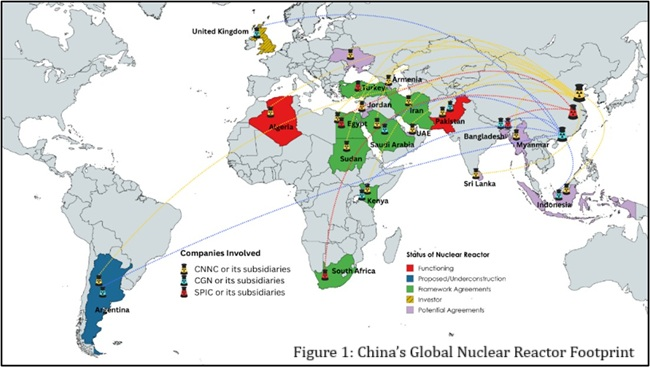
\includegraphics[width=0.82\linewidth]{assets/china-global-nuclear-reactor.jpg}
\caption{The Chinese footprint of nuclear reactors. Source: \jl{Vivekananda International Foundation}{https://www.vifindia.org/article/2025/august/08/How-Civilian-Nuclear-Energy-Is-Powering-China-s-Global-Strategy} (2025); reproduced for educational use.}
\label{fig:china_nuclear}
\end{figure}

\paragraph{(i)~The analytical lens: internationalization theory.}
The classical literature treats internationalization as a gradual, experience-driven process. The \jl{Uppsala model}{https://en.wikipedia.org/wiki/Uppsala_model} describes firms expanding in small steps, beginning with markets of low ``psychic distance'' and deepening commitment as knowledge accumulates; its revision recasts the central obstacle as the ``liability of outsidership'' --- being outside the relevant business network --- which is overcome through relationship-building.\cite{johanson_vahlne2009} Dunning's \jl{eclectic (OLI) paradigm}{https://en.wikipedia.org/wiki/Eclectic_paradigm} explains \emph{where} and \emph{why} firms invest abroad in terms of ownership, location and internalization advantages.\cite{dunning2000} A second wave corrects these models for emerging-market multinationals: Luo and Tung's \jl{springboard}{https://en.wikipedia.org/wiki/Springboard_Theory} perspective argues that such firms expand internationally to acquire strategic assets and to bypass constraints at home,\cite{luo_tung2007} while Mathews' ``dragon multinationals'' framework describes accelerated, partnership-based catch-up through linkage, leverage and learning.\cite{mathews2006} For Chinese firms specifically, outward investment is also shaped by state ownership and policy direction rather than firm-level advantage alone.\cite{buckley2007} The lens explains motives and process; it does not, by itself, tell us what a reactor export actually consists of.

\paragraph{(ii)~The load-bearing layer: the spectrum of deal structures.}
China's deliberate nuclear ``going-global'' strategy\cite{kenderdine2016} plays out across a spectrum of deal structures, from least to most integrated, and each point on it has a real exemplar. The dominant form is the \emph{turnkey export financed by a sovereign loan}: China designs, builds and finances the plant, while the host owns and operates it afterward and repays the debt. Pakistan's Karachi units~2 and~3 --- two Hualong One reactors supplied and built by CNNC --- are the model case, financed overwhelmingly by Chinese concessional lending (a China Eximbank preferential loan of about USD~6.5~billion against a project cost near USD~9.6~billion).\cite{wnn_karachi,aiddata_kanupp} The enabling feature, and the one a thesis should foreground, is \emph{state-backed concessional finance}: generous government support lets a state-owned enterprise offer terms no private firm could, so the host receives a plant it could not otherwise afford and China gains a multi-decade strategic foothold. Further along the spectrum lies the \emph{build--own--operate / equity} structure, in which China co-invests and shares operating revenue rather than simply building and leaving --- as China General Nuclear does with its roughly one-third stake in the United Kingdom's Hinkley Point~C --- a form reserved for partners able to co-invest.\cite{wnn_china} Most integrated is the \emph{localization or manufacturing joint venture}, in which the host's own industry shares in construction through local content, technology transfer and jobs --- increasingly the price of political acceptability for newcomer countries.

\paragraph{(iii)~Where SNERDI and Ye Cheng sit.}
SNERDI is the design institute behind SPIC's CAP1400 (``Guohe One''), an enlarged, Chinese-IP derivative of the AP1000.\cite{wnn_china} The brand passed the \jl{IAEA}{https://www.iaea.org/} Generic Reactor Safety Review in 2016 --- a review of the quality of the safety documentation, not a licence --- which SPIC presents as a foundation for international competition, and the company is now promoting its Gen-III technology to Turkey and South Africa, with early front-end engagement in Brazil and a nuclear-engineering training relationship with South Africa's Necsa.\cite{powermag_cap1400,wnn_china,snerdi_intl} This places SNERDI's contribution --- and therefore Ye Cheng's --- at the \emph{technology-and-licensing} end of an export deal: design suitability, safety-case localization and technical feasibility for a given country, rather than the financing or diplomacy that close it. That scoping is borne out by Ye Cheng's own account: his role in these projects was technical, including the submission of CAP1400-related technical documentation and the delivery of training in the South Africa engagement --- which both confirms the technology-and-licensing framing above and corroborates the Necsa training relationship from a primary source.

\paragraph{(iv)~The honest evidence base: success and failure.}
A credible Case~3 must reckon with how thin the export record actually is. The turnkey model has so far replicated only in Pakistan; no CAP1400 has yet been built as an export, and the flagship Latin-American attempt collapsed. Argentina's Atucha~III --- a 1.2~GW Hualong One signed in 2022 at about USD~8.3~billion with China offering to finance 85\% --- stalled when Argentina, amid hyperinflation, demanded full financing.\cite{diplomat_argentina,neutronbytes2026} The recurring barriers are analytically clean: the limits of concessional finance, the buyer's own capacity to fund its share, and the political continuity a multi-decade build needs to survive electoral turnover. The contrast --- Pakistan succeeds, Argentina fails --- is precisely the evidence base that turns Case~3 from a promotional account of ``how China sells reactors'' into an analysis of \emph{when and why the model works}.

\paragraph{(v)~Synthesis, framework decision, and gap.}
The thesis therefore does not assert a single model. It maps the spectrum of structures, uses the internationalization theories to explain which structure suits which kind of partner (capacity to pay, political risk, localization demand), and asks what arrangement could realistically bring Chinese fission now --- and spherical-tokamak fusion later --- to Brazil and South Africa, with SNERDI's CAP1400 engagements and the Pakistan/Argentina contrast as the evidence. The theories supply the ``why'' (springboard and linkage motives, Uppsala gradualism, state-directed investment); the deal structures supply the ``what''; and the gap is that no study joins the two for a Chinese energy technology aimed at these specific markets --- still less for fusion, whose internationalization is entirely prospective. Here the proposal states its central analytical question: \emph{under what buyer-side conditions} a Chinese reactor export succeeds. Read across the five cases, four factors recur --- demand intensity (high for Pakistan, South Africa and Turkey; low for Brazil, already near 90\% clean; undercut by crisis in Argentina), financing capacity (China financed roughly 82\% in Pakistan, whereas Argentina could not fund its share), institutional and regulatory continuity (South Africa's 2{,}500\,MW determination was withdrawn under legal challenge; Argentina's policy whipsawed across administrations), and localization and technology transfer. The fourth factor is decisive for political durability, and it is exactly the layer SNERDI occupies --- so Ye Cheng's actual work answers one of the four conditions rather than standing beside them. As decarbonization lifts baseline demand, the first factor only strengthens, leaving financing, continuity and localization as the binding constraints --- which is where China's concessional finance and SNERDI's localization model become decisive, for fission now and for any prospective fusion export later. A further question --- genuinely open, and independent of any single case --- is whether fusion is \emph{easier} to sell abroad than fission at all: because a fusion plant carries no fissile fuel and breeds no weapons-usable plutonium in normal operation, it falls largely outside the fission safeguards regime, which could lower host-country and nonproliferation resistance; yet that same first-of-a-kind profile may \emph{deepen} the technological-dependence dimension (tritium supply, breeding-blanket know-how, and decades of vendor lock-in), so whether fusion's \emph{net} reception exceeds fission's is itself a question this framework is built to test.\cite{fusion_nonprolif} On the SNERDI-specific particulars --- the stage each engagement reached, the structure contemplated, and the barriers met in Brazil, South Africa and Turkey --- Ye Cheng's initial guidance is that the three engagements are broadly comparable in character; their finer detail will be developed with his fuller input as the thesis proceeds, the published literature and public record carrying the proposal in the meantime.

\bigskip

\phantomsection\addcontentsline{toc}{section}{c.~~Purpose of the Research}\section*{c.~~Purpose of the Research}
The purpose of this research is, fundamentally, to write a practical ``how-to'' blueprint for accomplishing TUNEM's stated mission: to prepare global nuclear-energy managers capable of connecting China's nuclear-energy ambitions to the development needs of their own countries. This thesis is aimed squarely at the engineer-entrepreneur who wishes to internationalize Chinese fusion energy --- the founder who, in a venture's early life, \emph{is} its manager, and so is precisely the engineer-and-manager TUNEM exists to train --- and it seeks to reconstruct, end to end, how spherical-tokamak fusion is moved from a laboratory device toward a commercial and international reality, and to distil from that account a transferable pathway others can follow. The significance is therefore not primarily one of technical novelty but of \emph{social benefit and global energy cooperation}: clean, abundant baseload power is among the most consequential levers for development in the Global South, and a viable route to deploy it --- through partnership rather than extraction --- directly serves both China's energy diplomacy and the shared development of its partner nations in Latin America and Africa. The overarching question is: \emph{what does it take to carry spherical-tokamak fusion from device to commercial and international reality in China, and what generalizable pathway connects building the reactor, commercializing the venture, and internationalizing the business so that it delivers real benefit abroad?} It is pursued through three sub-questions, one per case and read through a common \textbf{Capabilities $\rightarrow$ Commercialization $\rightarrow$ International Markets} framework: (SQ1) which physics and engineering choices define the compact spherical-tokamak reactor embodied by SUNIST-2; (SQ2) how that capability becomes a viable, financed and regulated enterprise in Startorus Fusion; and (SQ3) which internationalization structures could carry a Chinese energy technology of this kind abroad --- for the mutual benefit of China and host nations --- in light of SNERDI's experience.

\phantomsection\addcontentsline{toc}{section}{d.~~Expected Results and Research Scheme}\section*{d.~~Expected Results and Research Scheme}
The research scheme is a unified three-case study whose cases are deliberately staged: SUNIST-2 (build), Startorus (commercialize), and SNERDI's international energy work (internationalize). The expected results are four. First, a \emph{physics-guided design philosophy} that maps reactor design choices --- magnetic field strength, plasma shape, heating strategy and pulse scheme --- to plasma performance, engineering and material constraints, and economic trade-offs; this synthesis, which connects the specialist systems-design literature\cite{process2020} to the commercial questions of Cases~2--3, is the analytical contribution of Case~1. Second, a firm-level reconstruction of Startorus's commercialization logic in which financing is one input among capabilities, products, profitability, regulation and state alignment. Third, a comparative analysis of internationalization structures (turnkey-plus-sovereign-loan, build--own--operate equity, and localization joint venture) and of which suits which partner, anchored on SNERDI's CAP1400 engagements and the Pakistan/Argentina contrast. Fourth, a cross-case synthesis --- the ``blueprint'' --- that links the three. A light, transparent quantitative layer supports each case: the published spherical-tokamak cost scaling ($P_{\mathrm{fus}}\propto R^{3}B^{4}\beta^{2}$) for Case~1, a funding-versus-milestone trajectory for Case~2, and a weighted country-entry comparison for Case~3.

\phantomsection\addcontentsline{toc}{section}{e.~~Research Method and Its Demonstration}\section*{e.~~Research Method and Its Demonstration}
This thesis adopts a \emph{mixed-methods, embedded single-case (process) study} (Yin\cite{yin2018}): because the three ``cases'' are sequential stages of one chain rather than independent replications, the design is processual, not Eisenhardt-style comparative replication\cite{eisenhardt1989}. Each stage is examined with the method it demands, the three integrated through the common Capabilities $\rightarrow$ Commercialization $\rightarrow$ International Markets framework. The three cases are not independent --- SUNIST-2 (capability), Startorus (commercialization) and SNERDI's international work (markets) form a single capability-to-market chain, which is the case-selection logic --- and a uniform written \emph{case protocol} interrogates each with the same questions (what is the capability, what bounds it, what is demonstrated versus still unproven, and what is the strategic logic), keeping them commensurable. Three methodological strands run in parallel.

\emph{Strand A --- analytical reconstruction (Case~1).} The reactor case is \emph{derived}, not summarised; the method is first-principles \emph{analytical reconstruction} --- taking the design-determining physics that specialist sources compress or assume and rebuilding it transparently, at a rigour appropriate to a reader who knows the mathematics but not the fusion. The thesis commits to deriving from first principles the \jl{Lawson}{https://en.wikipedia.org/wiki/Lawson_criterion} triple-product condition, the fusion-power scaling $P_{\mathrm{fus}}\propto R^{3}B^{4}\beta^{2}$, and the $\beta$--aspect-ratio relation that motivates the spherical tokamak; for the bootstrap closure it derives the \emph{geometric} core --- the trapped-particle fraction $\propto\sqrt{\epsilon}$ from banana-orbit geometry, hence $f_{bs}\propto\sqrt{\epsilon}\,\beta_{p}$ --- while \emph{sourcing} the fitted neoclassical coefficient, and Freidberg's $0.44$, to the primary literature; the \emph{empirical} operational limits it does not claim to derive at all (the Troyon $\beta$ and Greenwald density limits) are presented with provenance to their sources. The reconstruction follows the analytical template of Freidberg, Mangiarotti and Minervini,\cite{freidberg2015} draws its governing equations from the standard texts (Freidberg; Wesson; Lamarsh; Duderstadt) cited to section, and is \emph{validated} by first reproducing the published conventional-tokamak closure result --- the kink and bootstrap failure, $0.44<0.84$ --- before extending the same apparatus to the spherical tokamak. The rigour standard is that every relation is either derived or sourced to its primary derivation, with no asserted number lacking provenance. Here the author's mathematics background \emph{is} the method: the contribution is derivational accessibility, not new physics. As a worked demonstration, the cost-driving power scaling follows in a few steps: the fusion power density is $p_{\mathrm{fus}}\propto n^{2}\langle\sigma v\rangle$, and near reactor temperatures $\langle\sigma v\rangle\propto T^{2}$, so $p_{\mathrm{fus}}\propto(nT)^{2}\propto p^{2}$ in the plasma pressure $p$; since $\beta\equiv 2\mu_{0}p/B^{2}$ gives $p\propto\beta B^{2}$, this becomes $p_{\mathrm{fus}}\propto\beta^{2}B^{4}$, and multiplying by a plasma volume $\propto R^{3}$ yields $P_{\mathrm{fus}}\propto R^{3}B^{4}\beta^{2}$.

\emph{Strand B --- qualitative comparative case analysis (Cases~2 and~3).} The same protocol is applied, with evidence triangulated from three sources: peer-reviewed and technical literature; archival and quantitative records (funding rounds, device parameters, export-deal terms); and \emph{semi-structured} interviews, against a written interview guide, with the two principals --- Prof.\ Tan Yi for Cases~1--2 and Ye Cheng for Case~3. Advisor testimony is treated as \emph{enrichment, not foundation}: every case stands on public and published sources, interview material deepening but never carrying it --- as in b.3, where Ye Cheng's initial input enriches the public-source account without replacing it. Validity rests on triangulation, the uniform protocol, an explicit chain of evidence (every factual claim traced to a cited source --- the per-section citation audits already assembled \emph{are} that chain), and member-checking by returning drafts to the advisors.

\emph{Strand C --- light quantitative modelling.} Each case carries one transparent, reproducible model: the cost scaling $P_{\mathrm{fus}}\propto R^{3}B^{4}\beta^{2}$ and a breakeven check (Case~1), a funding-versus-milestone trajectory (Case~2), and a weighted country-entry comparison (Case~3). The first two rest on real scalings and data; the third is a \emph{structured qualitative} ranking whose weights are openly subjective and sensitivity-tested, not a predictive metric. All are illustrative, with assumptions made explicit.

The design fits both subject and author: a thesis about strategy and decisions suits the case-study tradition, while the analytical and quantitative strands let a mathematically-trained author contribute rigour through derivation and modelling. The contribution is the \emph{integration} --- carrying a first-principles design interface through to the commercial and international questions --- not any single new result.

\phantomsection\addcontentsline{toc}{section}{f.~~Methods for the Key Points and Difficulties}\section*{f.~~Methods for the Key Points and Difficulties}
Seven difficulties are anticipated, each tied to a countermeasure in the method above. \emph{Integrating heterogeneous strands:} an analytical derivation and a qualitative case study could read as two disconnected theses, so the strands are kept distinct in execution and joined only at the framework level, each validated on its own terms. \emph{Rigour versus accessibility:} the Case-1 reconstruction must satisfy a specialist on rigour and a non-specialist on clarity, so each relation is built from intuitive, geometrically-motivated steps, sourced to its primary derivation, and checked against published analytical results. \emph{The author's non-engineering background --- reframed as a methodological choice:} a mathematician reconstructs physics by \emph{deriving} it rather than by prior engineering training, which is the analytical-reconstruction method itself; rigour comes through derivation, with Prof.\ Tan Yi's verification as the check. \emph{Primary-data access:} advisor interviews cannot be assumed, so every case stands on public and published sources, interview input being enrichment (as with Ye Cheng's initial guidance, now folded into b.3 atop the public record). \emph{Cross-case comparability:} the single Capabilities$\rightarrow$Commercialization$\rightarrow$International Markets framework and the uniform case protocol keep three very different cases commensurable. \emph{Honesty of claims:} the internationalization case foregrounds failure (Argentina) beside success (Pakistan), and the quantitative models stay transparent and illustrative, not predictive. \emph{Positionality --- the advisors are also the subjects:} the two interviewees are themselves the protagonists of the cases (Prof.\ Tan Yi founded the Case-2 venture; Ye Cheng led the Case-3 deals), which risks an over-favourable account, so advisor testimony is treated as fact to be triangulated against independent and, where possible, critical sources; member-checking verifies accuracy rather than seeks endorsement; and the counterweights already built in --- foregrounding failure (Argentina) and claiming none of the engineering walls solved --- are retained as deliberate guards against boosterism.

\phantomsection\addcontentsline{toc}{section}{g.~~Overall Schedule}\section*{g.~~Overall Schedule}
\begin{center}
\begin{tabular}{|p{3.3cm}|p{11.0cm}|}
\hline
\textbf{Window} & \textbf{Milestone} \\ \hline
June 2026 & Lock title and research questions; submit the online topic form (by 26 Jun) and the proposal report (by 29 Jun); prepare the defense slides. \\ \hline
Early July 2026 & Proposal oral defense; incorporate committee feedback. \\ \hline
Aug--Oct 2026 & Deep literature; Case~1 and Case~2 data; interview Prof.\ Tan Yi; build the light quantitative models. \\ \hline
Nov 2026--Jan 2027 & Case~3 fieldwork; interview Ye Cheng; gather international-project data. \\ \hline
Feb--Mar 2027 & Cross-case synthesis (the ``blueprint''); draft chapters. \\ \hline
April 2027 & Full draft to advisors for review. \\ \hline
May 2027 & Revisions and submission. \\ \hline
June 2027 & Thesis defense. \\ \hline
\end{tabular}
\end{center}

\phantomsection\addcontentsline{toc}{section}{h.~~Date of the Final Defense}\section*{h.~~Date of the Final Defense}
The proposal will be defended orally in early July 2026. The final thesis defense is targeted for June 2027, subject to the department's scheduling.

\phantomsection\addcontentsline{toc}{section}{References}
\begin{thebibliography}{99}
\setlength{\itemsep}{1pt}

\bibitem{freidberg} J.~P.~Freidberg, \emph{Plasma Physics and Fusion Energy}. Cambridge University Press, 2007.
\bibitem{wesson} J.~Wesson, \emph{Tokamaks}, 4th ed. Oxford University Press, 2011.
\bibitem{lawson1957} J.~D.~Lawson, ``Some criteria for a power producing thermonuclear reactor,'' \emph{Proc.\ Phys.\ Soc.\ B} \textbf{70}, 6--10 (1957).
\bibitem{peng1986} Y.-K.~M.~Peng and D.~J.~Strickler, ``Features of spherical torus plasmas,'' \emph{Nucl.\ Fusion} \textbf{26}, 769 (1986). doi:10.1088/0029-5515/26/6/005.
\bibitem{sykes1997} A.~Sykes \emph{et al.}, ``High-$\beta$ performance of the START spherical tokamak,'' \emph{Plasma Phys.\ Control.\ Fusion} \textbf{39}, B247 (1997). doi:10.1088/0741-3335/39/12B/019.
\bibitem{sykes2018} A.~Sykes, A.~E.~Costley, C.~G.~Windsor \emph{et al.}, ``Compact fusion energy based on the spherical tokamak,'' \emph{Nucl.\ Fusion} \textbf{58}, 016039 (2018). doi:10.1088/1741-4326/aa8c8d.
\bibitem{costley2019} A.~E.~Costley, ``Towards a compact spherical tokamak fusion pilot plant,'' \emph{Phil.\ Trans.\ R.\ Soc.\ A} \textbf{377}, 20170439 (2019). doi:10.1098/rsta.2017.0439.
\bibitem{mcnamara2024} S.~A.~M.~McNamara \emph{et al.}, ``Overview of recent results from the ST40 compact high-field spherical tokamak,'' \emph{Nucl.\ Fusion} \textbf{64}, 112020 (2024). doi:10.1088/1741-4326/ad6ba7.
\bibitem{ono2015} Y.~Ono \emph{et al.}, ``High power heating of magnetic reconnection in merging tokamak experiments,'' \emph{Phys.\ Plasmas} \textbf{22}, 055708 (2015).
\bibitem{tanabe2015} H.~Tanabe \emph{et al.}, ``Electron and ion heating characteristics during magnetic reconnection in the MAST spherical tokamak,'' \emph{Phys.\ Rev.\ Lett.} \textbf{115}, 215004 (2015). doi:10.1103/PhysRevLett.115.215004.
\bibitem{nelson2024} A.~O.~Nelson \emph{et al.}, ``Characterization of the ELM-free negative triangularity edge on DIII-D,'' \emph{Plasma Phys.\ Control.\ Fusion} \textbf{66}, 105014 (2024). doi:10.1088/1361-6587/ad6a83 (arXiv:2405.11082).
\bibitem{camenen2007} Y.~Camenen \emph{et al.}, ``Impact of plasma triangularity and collisionality on electron heat transport in TCV L-mode plasmas,'' \emph{Nucl.\ Fusion} \textbf{47}, 510 (2007).
\bibitem{tan_iaea} Y.~Tan, Z.~Gao \emph{et al.}, ``Recent progress on the SUNIST-2 spherical tokamak,'' 30th IAEA Fusion Energy Conference (FEC~2025), paper IAEA-CN-316/3327 (open access).
\bibitem{cheng2022} Z.~Cheng, Z.~Gao and Y.~Tan, ``Equilibrium design for the SUNIST-2 spherical tokamak,'' 21st International Spherical Torus Workshop (ISTW~2022), Beijing (open access).
\bibitem{li2025} X.~Li \emph{et al.}, ``Development of plasma burn-through simulation code and validation in SUNIST-2 and EAST,'' \emph{Nucl.\ Fusion} \textbf{65}, 066017 (2025). doi:10.1088/1741-4326/add1f0 (open access).
\bibitem{sunist_cn2004} L.~Zeng, Y.-x.~He and the SUNIST Team, ``Construction of the Sino-United Spherical Tokamak'' (in Chinese), \emph{Atomic Energy Science and Technology} \textbf{38}(6), 501 (2004). doi:10.7538/yzk.2004.38.06.0501.
\bibitem{tan_gao2010_cn} Y.~Tan and Z.~Gao, ``Measurement of the magnetic-probe outgassing rate in the SUNIST device'' (in Chinese), \emph{Nuclear Fusion and Plasma Physics} \textbf{30}(3) (2010).
\bibitem{tan_phd2009} Y.~Tan, ``Experimental study of non-inductive current start-up and sustainment on the SUNIST spherical tokamak'' (PhD dissertation, in Chinese), Tsinghua University, 2009.
\bibitem{sunist2design2025} SUNIST-2 Team, ``The preliminary design of SUNIST-2: a spherical tokamak,'' \emph{Fusion Eng.\ Des.} \textbf{212}, 114865 (2025). doi:10.1016/j.fusengdes.2025.114865.
\bibitem{sunist2control2024} SUNIST-2 Team, ``Preliminary progress of magnetic plasma control for the SUNIST-2 spherical tokamak,'' \emph{Plasma Phys.\ Control.\ Fusion} (2024). doi:10.1088/1361-6587/ae1533.
\bibitem{hender2007} T.~C.~Hender \emph{et al.}, ``Chapter~3: MHD stability, operational limits and disruptions,'' \emph{Nucl.\ Fusion} \textbf{47}, S128 (2007). doi:10.1088/0029-5515/47/6/S03.
\bibitem{boozer2012} A.~H.~Boozer, ``Theory of tokamak disruptions,'' \emph{Phys.\ Plasmas} \textbf{19}, 058101 (2012).
\bibitem{freidberg2015} J.~P.~Freidberg, F.~J.~Mangiarotti and J.~Minervini, ``Designing a tokamak fusion reactor---how does plasma physics fit in?,'' \emph{Phys.\ Plasmas} \textbf{22}, 070901 (2015). doi:10.1063/1.4923266 (open: osti.gov/biblio/1547016).
\bibitem{troyon1984} F.~Troyon, R.~Gruber, H.~Saurenmann \emph{et al.}, ``MHD-limits to plasma confinement,'' \emph{Plasma Phys.\ Control.\ Fusion} \textbf{26}, 209 (1984).
\bibitem{greenwald1988} M.~Greenwald, J.~L.~Terry, S.~M.~Wolfe \emph{et al.}, ``A new look at density limits in tokamaks,'' \emph{Nucl.\ Fusion} \textbf{28}, 2199 (1988).
\bibitem{kikuchi1990} M.~Kikuchi, ``Steady state tokamak reactor based on the bootstrap current,'' \emph{Nucl.\ Fusion} \textbf{30}, 265 (1990).
\bibitem{menard2016} J.~E.~Menard \emph{et al.}, ``Fusion nuclear science facilities and pilot plants based on the spherical tokamak,'' \emph{Nucl.\ Fusion} \textbf{56}, 106023 (2016). doi:10.1088/0029-5515/56/10/106023.
\bibitem{wurzel_hsu2022} S.~E.~Wurzel and S.~C.~Hsu, ``Progress toward fusion energy breakeven and gain as measured against the Lawson criterion,'' \emph{Phys.\ Plasmas} \textbf{29}, 062103 (2022).
\bibitem{keilhacker1999} M.~Keilhacker \emph{et al.}, ``High fusion performance from deuterium--tritium plasmas in JET,'' \emph{Nucl.\ Fusion} \textbf{39}, 209 (1999).
\bibitem{abushawareb2024} H.~Abu-Shawareb \emph{et al.} (Indirect Drive ICF Collaboration), ``Achievement of target ignition at the National Ignition Facility,'' \emph{Phys.\ Rev.\ Lett.} \textbf{132}, 065102 (2024).
\bibitem{abdou2006} M.~Abdou \emph{et al.}, ``Physics and technology conditions for attaining tritium self-sufficiency for the D--T fuel cycle,'' \emph{Fusion Eng.\ Des.} (2006).
\bibitem{zinkle_snead2014} S.~J.~Zinkle and L.~L.~Snead, ``Designing radiation resistance in materials for fusion energy,'' \emph{Annu.\ Rev.\ Mater.\ Res.} \textbf{44}, 241 (2014).
\bibitem{boozer2005} A.~H.~Boozer, ``Physics of magnetically confined plasmas,'' \emph{Rev.\ Mod.\ Phys.} \textbf{76}, 1071 (2005).
\bibitem{process2020} S.~I.~Muldrew \emph{et al.}, ``\,`PROCESS': systems studies of spherical tokamaks,'' \emph{Fusion Eng.\ Des.} \textbf{154}, 111530 (2020).
\bibitem{fia2025} Fusion Industry Association, \emph{The Global Fusion Industry in 2025} (Washington, DC, 2025).
\bibitem{xinhua2025} Xinhua, ``China sets up state-owned fusion energy company amidst push for inexhaustible clean power,'' 24~July 2025.
\bibitem{tan_interview_cn} ``Dialogue with Tsinghua's Tan Yi: controlled fusion need not wait another fifty years'' (in Chinese), Sohu, 2025.
\bibitem{chenrui_interview_cn} ``Interview with Chen Rui, CEO of Startorus Fusion'' (in Chinese), Sina Finance, 2024.
\bibitem{johanson_vahlne2009} J.~Johanson and J.-E.~Vahlne, ``The Uppsala internationalization process model revisited: from liability of foreignness to liability of outsidership,'' \emph{Journal of International Business Studies} \textbf{40}, 1411--1431 (2009).
\bibitem{dunning2000} J.~H.~Dunning, ``The eclectic paradigm as an envelope for economic and business theories of MNE activity,'' \emph{International Business Review} \textbf{9}(2), 163--190 (2000).
\bibitem{luo_tung2007} Y.~Luo and R.~L.~Tung, ``International expansion of emerging market enterprises: a springboard perspective,'' \emph{Journal of International Business Studies} \textbf{38}(4), 481--498 (2007).
\bibitem{mathews2006} J.~A.~Mathews, ``Dragon multinationals: new players in 21st-century globalization,'' \emph{Asia Pacific Journal of Management} \textbf{23}(1), 5--27 (2006).
\bibitem{buckley2007} P.~J.~Buckley \emph{et al.}, ``The determinants of Chinese outward foreign direct investment,'' \emph{Journal of International Business Studies} \textbf{38}(4), 499--518 (2007).
\bibitem{wnn_karachi} ``Karachi~2: final sign-off for first Hualong One export,'' World Nuclear News (2021); ``China formally hands over Karachi~2 Hualong One reactor to Pakistan,'' Nuclear Engineering International (2021).
\bibitem{aiddata_kanupp} AidData, ``China Eximbank provides \$3.618~billion preferential buyer's credit for Units~2 and~3 of the Karachi Nuclear Power Plant (KANUPP),'' \jl{china.aiddata.org}{https://china.aiddata.org/projects/41918/}.
\bibitem{wnn_china} World Nuclear Association, ``Nuclear Power in China'' (CAP1400 / Guohe One export promotion to Turkey and South Africa; CGN equity in UK projects), country profile, accessed 2026.
\bibitem{powermag_cap1400} ``China's CAP1400 clears IAEA safety assessment,'' POWER Magazine (2016); IAEA, Generic Reactor Safety Review of the CAP1400 design.
\bibitem{snerdi_intl} Shanghai Nuclear Engineering Research \& Design Institute, ``International,'' \jl{snerdi.com.cn/en/International}{https://www.snerdi.com.cn/en/International} (cooperation with Necsa, South Africa; Eletronuclear RFI, Brazil; Turkey delegation), accessed 2026.
\bibitem{diplomat_argentina} ``Why Argentina's nuclear power project with China has stalled,'' The Diplomat, December 2022.
\bibitem{fusion_nonprolif} ``Nonproliferation and fusion power plants,'' arXiv preprint arXiv:2207.14348 (2022).
\bibitem{neutronbytes2026} ``Why China came up short in nuclear exports,'' Neutron Bytes, February 2026.
\bibitem{kenderdine2016} T.~Kenderdine, ``China's nuclear industry goes global,'' The Diplomat, 2016 (the ``Nuclear Silk Road'' export strategy).
\bibitem{yin2018} R.~K.~Yin, \emph{Case Study Research and Applications: Design and Methods}, 6th ed. Thousand Oaks: Sage, 2018.
\bibitem{eisenhardt1989} K.~M.~Eisenhardt, ``Building theories from case study research,'' \emph{Academy of Management Review} \textbf{14}(4), 532--550 (1989).

\end{thebibliography}

\end{document}
